Durant le développement de nos différents clients, nous nous sommes rendus
compte que nous étions très limité par le temps de calcul. En effet,
la plupart de nos algorithmes n'étaient pas optimisés. Nous avons donc
eu recourt à du profilage

\subsection{Profilage et identification de zone critiques}
Après premier appel au profileur \textit{gprof} montré dans la Figure \ref{fig:gprof-find-neighbors}
, nous voyons déjà une première zone critique, \verb|find_neighbor_in_direction|.

\begin{figure}[H]
	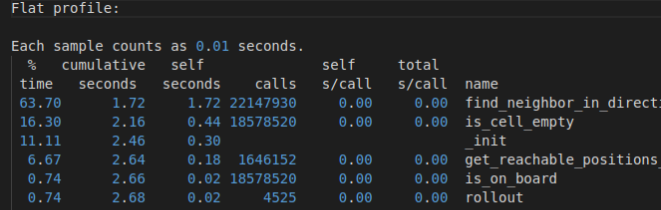
\includegraphics[width=\linewidth]{gprof_before}
	\caption{Résultat du profileur \textit{gprof} après exécution d'une itération MCTS}
	\label{fig:gprof-find-neighbors}
\end{figure}

On remarque que la fonction \verb|find_neighbor_in_direction| nous mange
toute la puissance de calcul. Cette fonction est appelée plus de 22 millions de fois, elle 
occupe 63.70\% du temps CPU et la somme de la durée prise par tous ses appels est égale à 1.72 secondes, ce qui est gigantesque
pour une seule itération de MCTS. Au moment du profile, la fonction \verb|find_neighbor_in_direction| avait le fonctionnement défini
dans l'algorithme \ref{alg:find_neighbor_before}. Sa complexité était au moins de $O(nombre\_sommets)$ soit $O(n)$. Nous voudrions une complexité
$O(1)$ idéalement vu le nombre d'appels à cette fonction.

\begin{algorithm}
	\Entree{M: matrice d'adjacence}
	\label{alg:find_neighbor_before}
\end{algorithm}